\section{Control of physics-based animation}
\label{sec:starSimulationControl}

As we mentioned in the introduction, computer were used for producing animations in two main ways. 
First, principles of traditional animation were adopted, leaving the animator to describe the key-frames that would bring life and style to characters. 
Second, physics was used to animate objects whose complexity in terms of scale and behavior would have been intractable for a single animator. 
Nowadays, these two use cases are only the extremities of a large spectrum. 
In between lies the control of physics-based animations which tends to take into account both user directions, that will bring life and style, and physics, that will handle the exciting complexity and dynamics of the physical behavior.
In this section, we illustrate the problem of simulation control and describe the main solutions proposed so far.
\subsection{Problem: The trials and errors process}
How to control a physics-based animation is an old problem in computer graphics. In order to understand the different problems that arise, it is good to start from the most naive way of controlling a physics-based animation: trials and errors. 

Let's say we have to design an animation of a ball launched on the ground that bounces two times before hitting the center of a target on the ground. 
The elastic behavior of the ball and the changes of speed make it a hard animation for a key-framing animator. 
Using physically-based simulation methods, the behavior takes some time to compute but can be easily solved.
As the simulation is an initial value problem, the whole behavior of the ball is dictated by the initial and boundary conditions of the simulation, the material parameters of the ball and the external forces that can be set to help guiding the animation. 
The trials and errors process consists in setting these conditions and parameters, running the simulation and correcting the parameters until the ball reaches the desired target (see Figure~\ref{fig:trialErrorProcess}). 
\begin{figure}[!h]
	\centering
	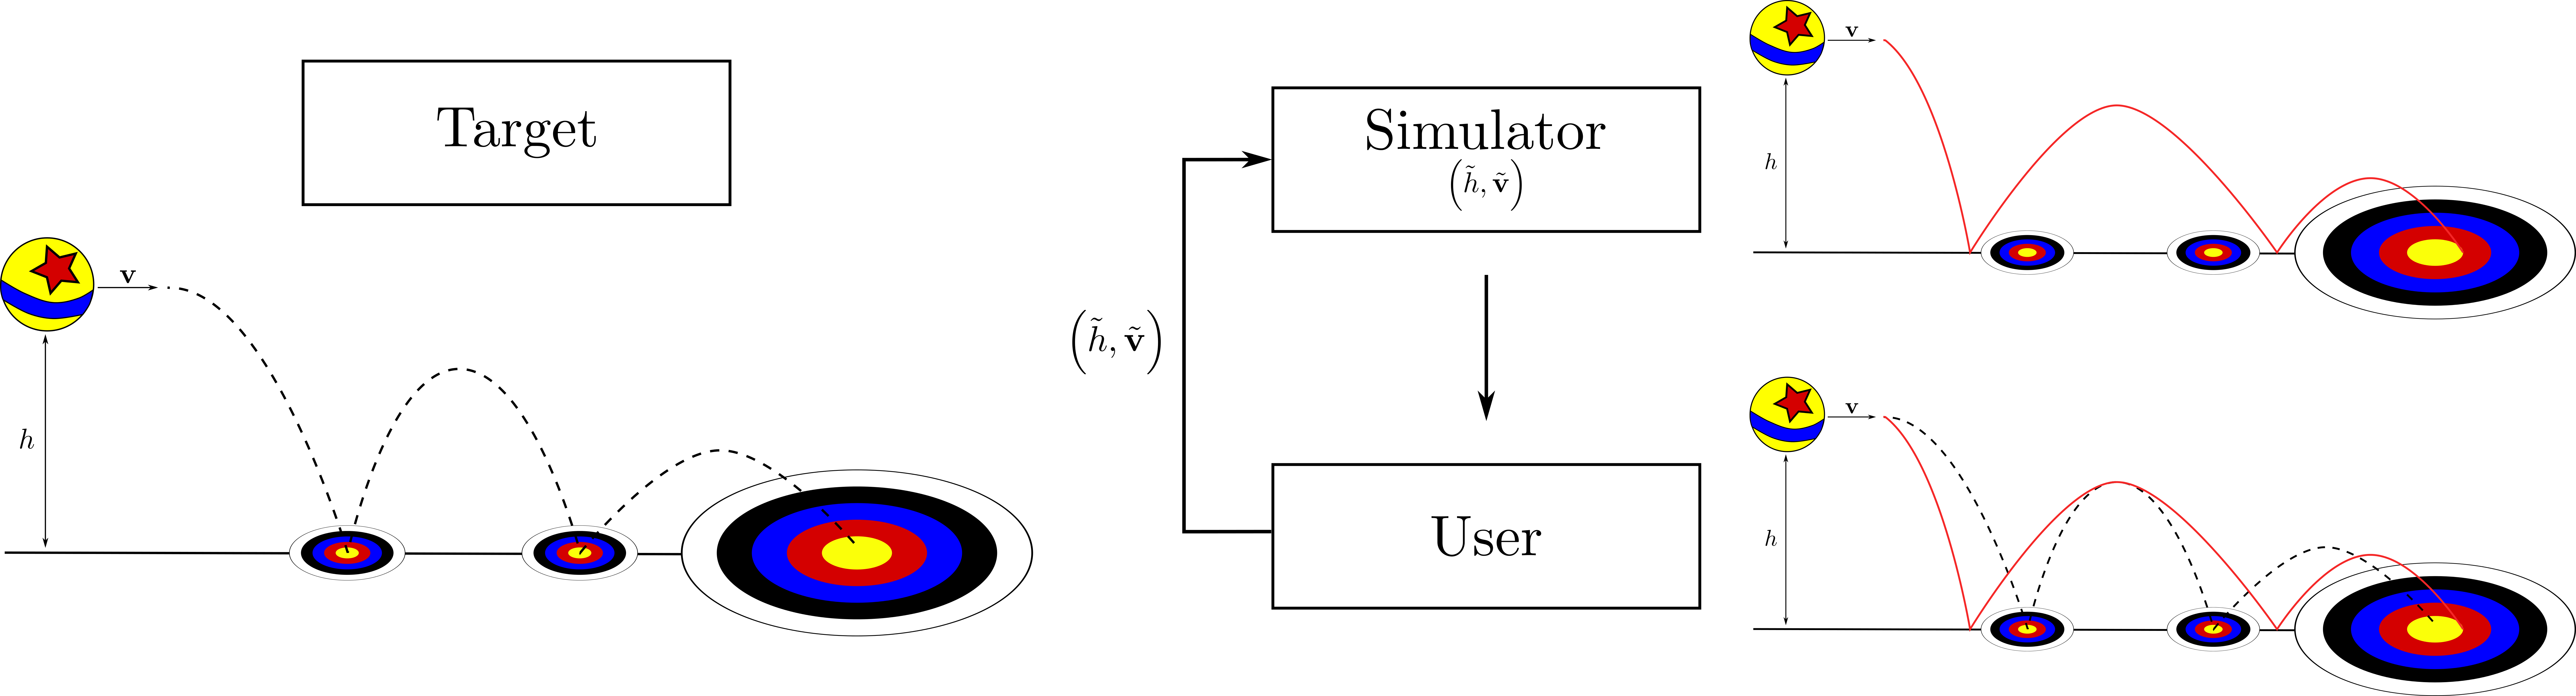
\includegraphics[width=\linewidth]{./images/simulationControl/trialError.png}
	\caption[STAR control: Trial and error process]{\label{fig:trialErrorProcess}Trial and error process. 
	The user runs successive simulations with different parameters such as the initial height $h$ and velocity $\mathbf{v}$ of the ball until it reaches a desired target.}
\end{figure}

There are mainly three constraints which make this task a nightmare:
\begin{itemize}
	\item Firstly, the computational time plays a major role. 
	This is obvious but still important to states. 
	A real-time simulation will allow the user to quickly explore parameters whereas an offline simulation might require days and days of tuning.
    Here, we can mention procedural tools which are generally much more efficient than simulation and therefore enable faster editing loops. Unfortunately they are often limited to overly restrictive models such as large open ocean surfaces~\cite{hinsinger2002,Tessendorf2004,jeschke2015water,horvath2015empirical}.
	\item Secondly, the control is indirect and, most of the time, based on unintuitive parameters which requires some expertise about the underlying physical model. The user cannot directly control the trajectory nor the shape of the object.
	\item Thirdly, many physics-based animations describe a non-linear behavior. Fluid animations are among them for instance. 
	This non-linearity makes it very hard to choose the right parameters. 
	Small changes can produce very different results making tedious to explore the range of possible behaviors and almost impossible to respect specific artistic directions such as timing, key positions, trajectories or shapes. 
	Also, it prevents the user from interactively controlling a low-resolution simulation and then achieve a similar behavior with the same parameters at a higher resolution.
\end{itemize}

\subsection{Space-time constraints paradigm}
A general approach for controlling a physics-based animation is to formulate it as an optimization under constraints: 
"\emph{Find the value of the parameters such that the physical behavior and user constraints are respected over the animation}" 
(see Figure~\ref{fig:spaceTimeConstraints}).
\begin{figure}[!h]
\centering

\includegraphics[width=\linewidth]{./images/simulationControl/spaceTimeConstraints.png}
\caption[STAR control: Space-time constraints]{\label{fig:spaceTimeConstraints} Space-time constraints. 
An optimization problem is defined to find the value of the parameters which solve the equations of motion while respecting constraints defined by the user.
In this example, the parameters are the initial height $h$ and velocity $\mathbf{v}$ of the ball and the constraints are the position of the ball at different time.
The ball has a mass of $1\kilo\gram$ and is only submitted to the gravity $\mathbf{g}$.}
\end{figure}

Four challenges arise, what are the parameters we want to control, what are the user constraints, how to formulate them and finally how to numerically solve the problem. 
Witkin and Kass were among the first to introduce this formulation to the computer graphics community in their pioneer work \emph{Space-time constraints}~\cite{Witkin1988}.

\subsubsection{Parameters}
The most common parameters are the positions of the material samples and the external forces.
A common drawback of using external forces is that the necessary changes may become highly unrealistic.
As an alternative, Coros et al.~\cite{Coros2012} proposed to adapt the rest shape of the object from one frame to another in order to induce internal forces that would match the user goals.
When large deformation occurs it is possible that the computed solution is at the limit of the deformation that the object can reach. In order to enforce the optimization, Li et al.~\cite{Li2014} proposed to optimize material parameters as well. 

\subsubsection{Constraints}
Position, velocity and density are among the constraints that are most often used for controlling an animation. 
Of course, they depend on the simulated object: rigid, solids, smoke, liquid, etc. 
Certainly, position constraints are the most intuitive for the user as they can be specified using key-frames. 
However, designing a key-frame for a highly elastic object or viscous materials might be extremely hard to achieve. 
Here there is a direct link to the works about surface modeling which propose to deform naturally an object~\cite{Sorkine2007, Hildebrandt2011}. 
In some cases, these deformation tools can be seen as a local static simulation of the object that computes its deformation from a displacement induced by the user. 
For elastic objects, such deformation tool has been proposed by Barbic et al.~\cite{Barbic2012}.
For liquids, Pan et al.~\cite{Pan2013} propose an interactive method to deform wave shapes by sketching their profiles. 
Thus, direct spatial deformation is made possible. 
Both fits in the framework of surface modeling deformation. 
The only difference is that the functions which are minimized are directly derived from the internal forces acting on the object. 
These methods are particularly useful when interactively editing an animation, specially when they are combined with high level deformation tools such as sketching.

\subsubsection{Numerical solution}
In their work, Witkin and Kass~\cite{Witkin1988} dealt with small systems and short simulation period.
Therefore, they could afford to directly solve the optimization problem, meaning that at each iteration a whole simulation would be computed. For instance, small rigid bodies simulation could be interactively designed through this approach~\cite{Popovic2000,Popovic2003}. For complex models and large simulation time, this approach is intractable. Windowing methods allowed to restrict the optimization to the space-time range of interests~\cite{Cohen1992}. In their work~\cite{McNamara2004} proposed to use the adjoint method to efficiently compute gradients in liquid simulation thus improving the performance of the optimization. The approach was also used by Wojtan et al.~\cite{wojtan2006keyframe} for handling large particle systems. For elastic bodies, the use of reduced model allowed to achieve speed-ups of several order of magnitude, thus allowing to interactively edit a physics-based animation~\cite{Barbic2012,Hildebrandt2012,Hahn2012}. Since, this approach has been further improved to be faster~\cite{Schulz2014} and to deal with large deformations~\cite{Li2014}.

\subsection{Applications \& Alternatives}
The strength of the space-time constraints paradigm relies on its very general definition. Therefore, a large number of applications and methods can be seen as offsprings of this approach. In the following, we distinguish different applications of physics-based animation control and present alternatives to the above methods.

\subsubsection{Enriching an animation with physics}
Given a full animation, a simulation is run in order to enhance the input animation with detailed physically-based secondary motions. This approach was successfully applied to enhance character animation with wrinkles and folds of their skin by Bergou et al.~\cite{Bergou2007}. In their work, they compute the dynamics of thin shells on top of the animation by using a multi-resolution approach. In fluid animation, details enhancing brings a lot of attention as it would be easier to set up low resolution simulation and add details on top of it without loosing the global behavior. A nice approach was proposed by Mercier et al.~\cite{Mercier2015} where they solve a Lagrangian wave simulation only at the surface of the low resolution simulation.

\subsubsection{Guiding a simulation with animation data}
A large number of methods propose to guide a simulation without the need of an expensive optimization problem. 
Generally these methods propose to use external forces that are automatically computed from the user inputs such as key-frames.
One of the first approach of this kind was proposed by Lamouret and Cani~\cite{Lamouret1996}.
This approach was later extended to more involved inputs such as simulation data.
In the case of fluid, user-defined velocity field~\cite{Kim2006:SmokeControl}, distance fields~\cite{Yang2013} and control particles~\cite{Thurey2006:FluidControl,Madill2013} were proposed to control the trajectory of fluid animation.
Still in the same idea, there are many methods which propose to guide the behavior of an object using geometric proxies which are easier to control for an artist than simulation data. For example, artists can use a triangle mesh to specify a target shape which will act as an attractor by adding artificial attraction forces based on the distance to the mesh surface. 
Such approaches have been successfully developed to drive smoke~\cite{Fattal2004,Hong2004,Shi2005a} and liquid simulations~\cite{Shi2005b,Raveendran2012}.
Taking this strategy further, the geometric proxies themselves can be defined by a low-resolution fluid simulation. 
To achieve this, the artist quickly sets up a coarse simulation and uses the output geometry to guide the main features of a full resolution simulation.
Several approaches modify a high-resolution smoke simulation using optimization~\cite{Nielsen2009,Nielsen2010}, patterns extracted as skeleton~\cite{Yuan2011}, or sparse sampling~\cite{Huang2013}.
For liquid simulations, Nielsen and Bridson~\cite{Nielsen2011} propose to restrict the high resolution simulation to a thin layer around a guiding coarse animation.
Although each of these approaches are able to successfully guide an animation, they do not enable direct control of the resulting animation. Designing precise timing or feature scaling would therefore still require iterative trial-and-error steps to converge toward a desired animation.

\subsubsection{Example-based simulation}
Instead of controlling the trajectory of an object, one might want to control how it deforms when it collides with other objects. 
In exampled-based simulations, a set of examples that represent the desired deformations is used to build a space of preferred deformations from where internal forces will be deduced. This method was first introduced by Martin et al.~\cite{Martin2011} for elastic deformations. Jones et al.~\cite{Jones2016} propose a similar method to easily incorporate plastic deformations in rigid bodies simulations.

\subsubsection{Animation sampling}
In multibody systems, the space-time constraints paradigm can hardly be used. In cause, the large number of discontinuous contacts events which makes the optimization problem particularly difficult to solve. In contrast, multibody simulators are particularly fast, so fast that it is possible to run in parallel a large number of simulations. In their work,~\cite{Chenney2000}~and~\cite{Twigg2007} exploit this performance to sample the space of parameters of an animation and thus finding those which satisfy the user constraints.

\subsubsection{Animation editing} 
In contrast with simulation control, animation editing consists in deforming in space and time the output of a simulator without the need to re-simulate.
Closely related to surface modeling it has to take into account the temporal dimension and its relation with space in order to propose new editing tools. 
In these approaches, finding a natural way to deform an animation and ensuring temporal consistency are amongst the main challenges.
Very few methods have been proposed whereas it represents a much faster approach to edit animations.
Among the most interesting approaches, Pighin et al.~\cite{Pighin2004} propose to build a space-time parametrization of a smoke animation using advected radial basis functions. The parametrized data are then deformed using a trajectory-based editing tool.
Schpok et al.~\cite{Schpok2005} proposed to extract and parametrize features such as vortices, uniform advection, sinks and sources to allow the user to modify the parameters in a smoke simulation.
For animations of liquid, Raveendran et al.~\cite{Raveendran2014} propose a semi-automatic method to match two animations and smoothly interpolate between them. 
This approach allows to quickly explore parameter space such as boundary conditions or viscosity parameter and then to produce a large number of new animations without the need for re-simulation.

\subsection{Conclusion on simulation control}

All the methods mentioned above make a trade-off between realism and control.
On one hand, realism requires a high computational cost and makes methods such as space-time constraints unattractive for interactive use.
On the other hand, giving the user full control may introduce unphysical and unpleasant behavior.
Very few works explored the edit of an existing animation and how to extend classical modeling techniques to animated content.
We think that this approach would allow to interactively design physics-based animation without the need to re-simulate.
In Chapter~\ref{chap:fluidsculpting}, we will present a system for the design of fluid animation based on this idea.
